\begin{center}
    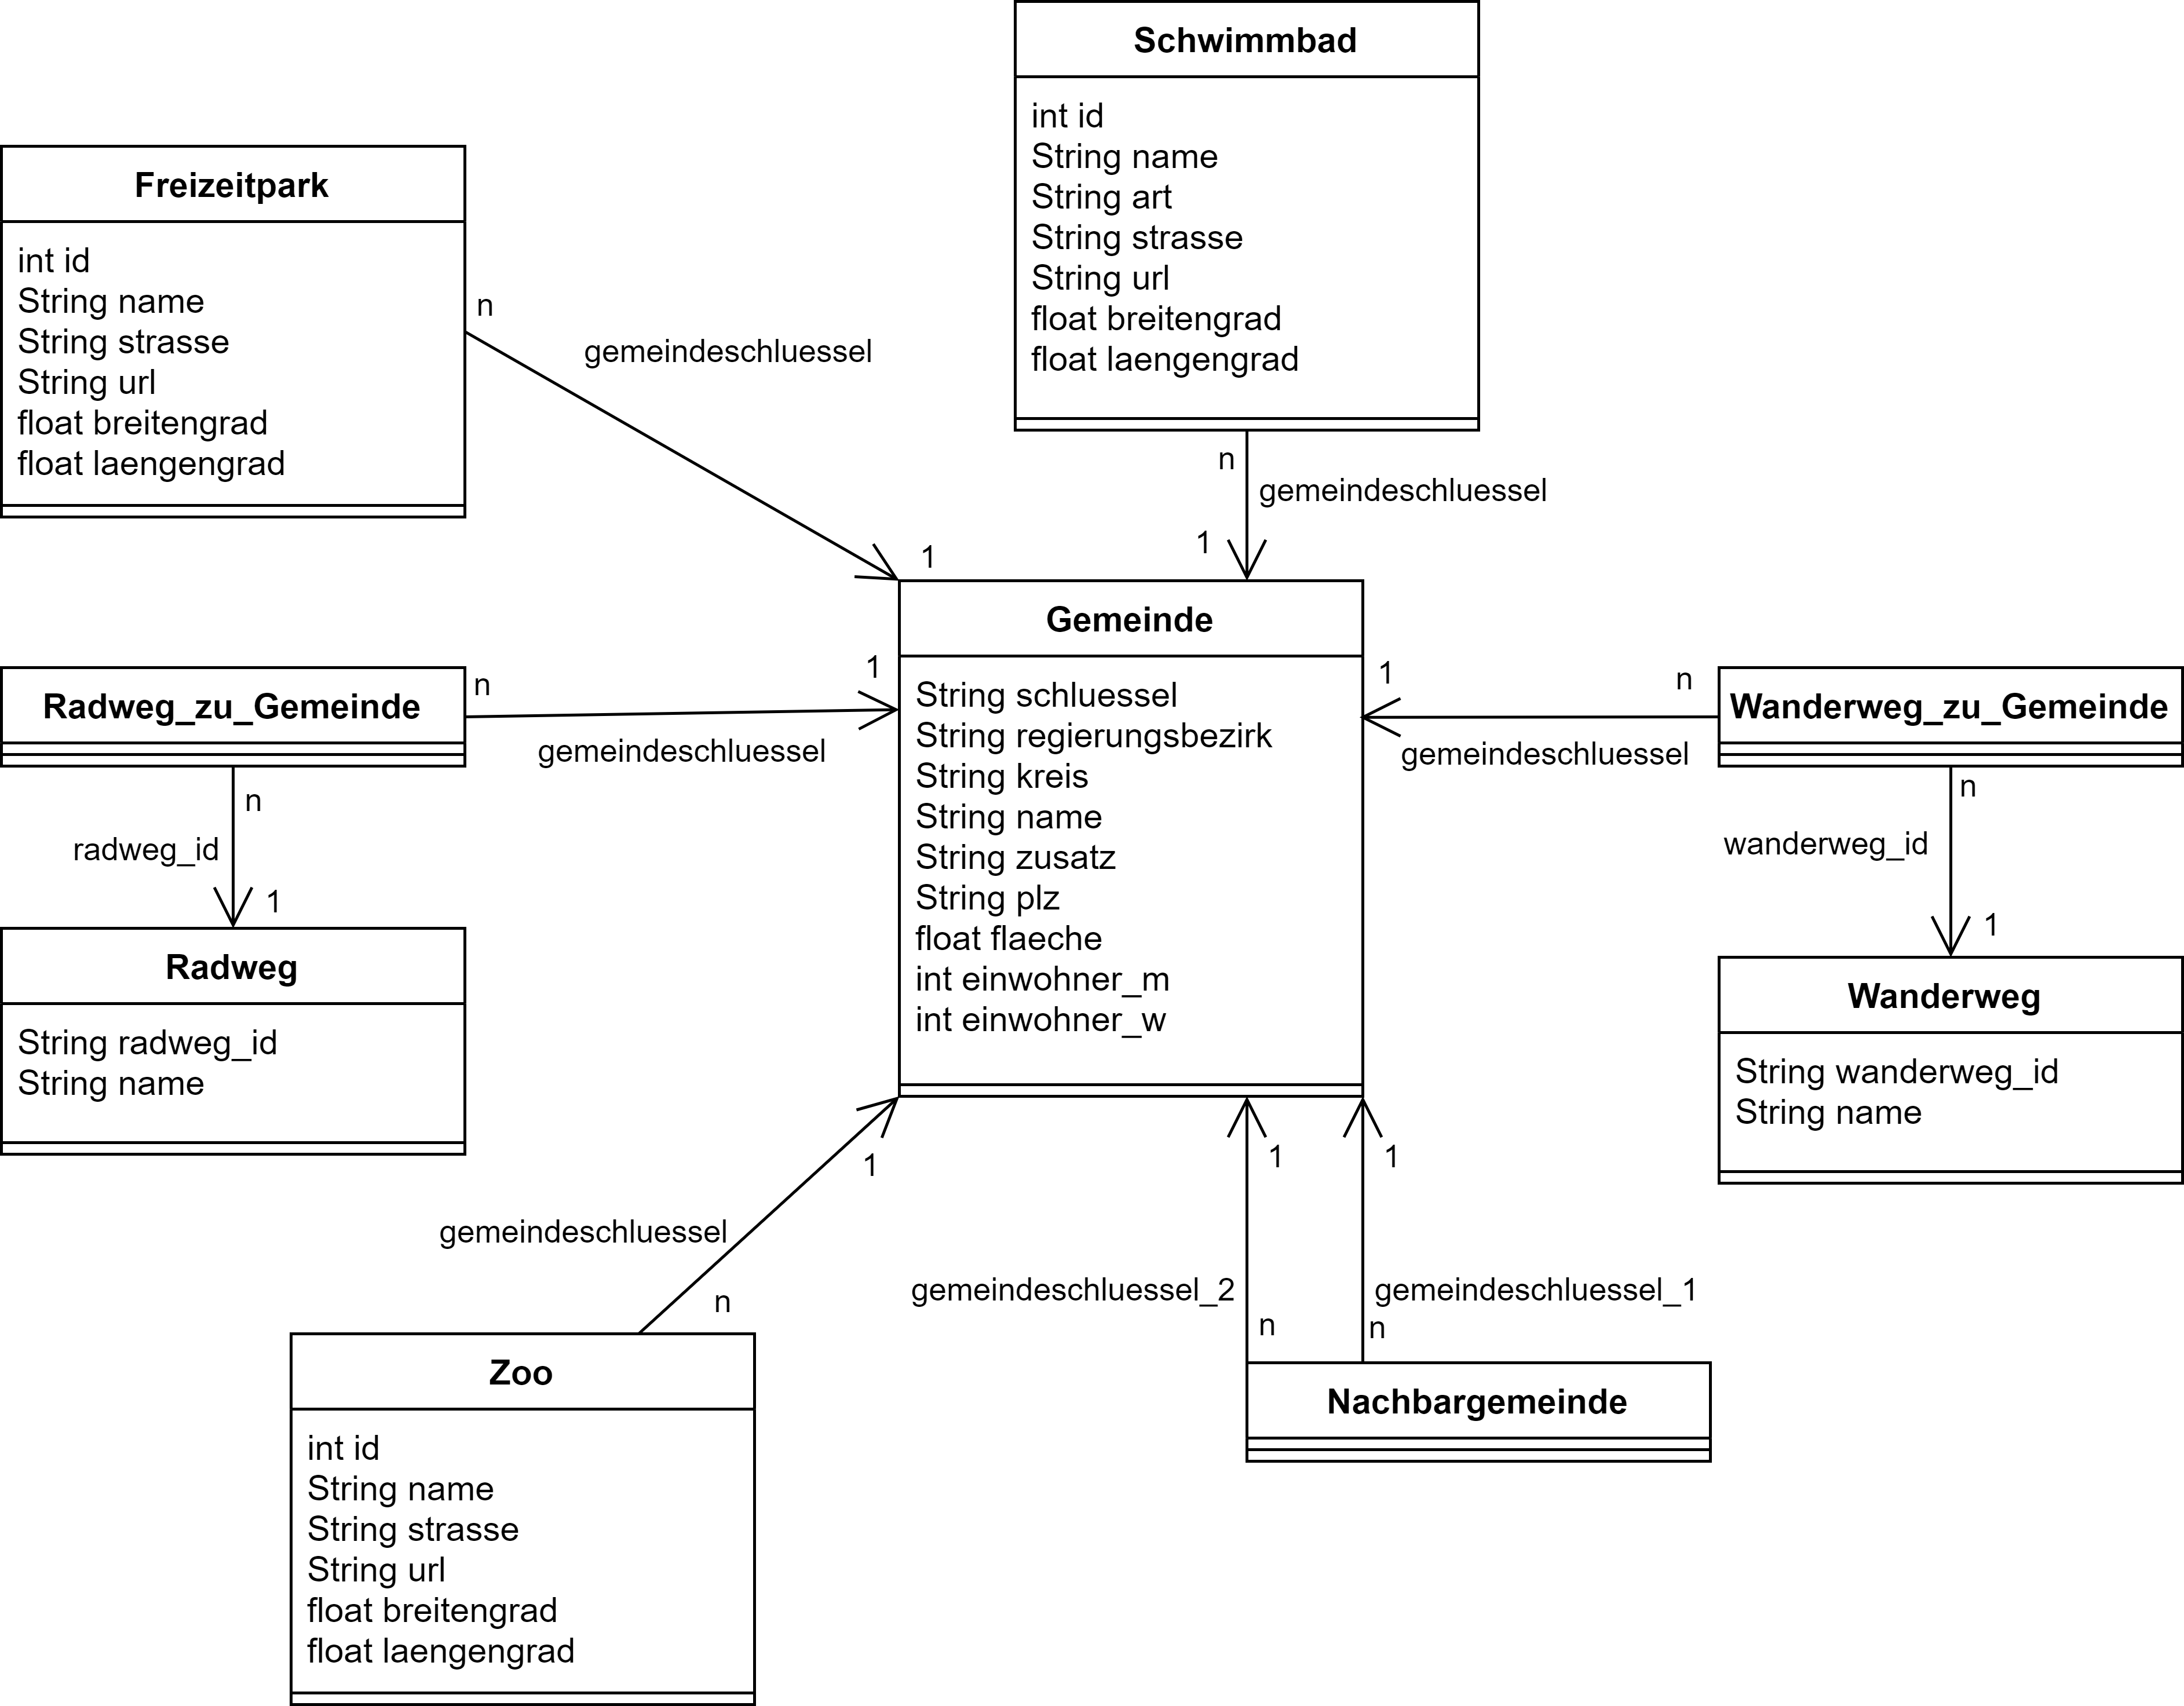
\includegraphics[width=\textwidth]{Aufgaben/img/Bayern_DB.png}
\end{center}

\Aufgabe{Aufgaben}{

Alle Aufgaben beziehen sich auf die Datenbank oben. Eine Online-Version gibt es unter \url{www.dbiu.de/bayern/}.

Gib immer genau die geforderten Daten aus und nicht mehr. Sortiere nicht, wenn du nicht dazu aufgefordert wirst.

\vspace{1cm}


Verändere die SQL-Abfrage so, dass die Namen und Internetadressen (=url) aller Zoos und der Name und Regierungsbezirk der jeweiligen Gemeinde ausgegeben wird:

\vspace{0.3cm}

\large
\emphBlue{SELECT Zoo.name, Gemeinde.name} \LoesungLuecke{,Gemeinde.regierungsbezirk, Zoo.url}{8cm}\\\vspace{0.5cm}
\emphBlue{FROM Zoo, Gemeinde}\\
\LoesungLuecke{WHERE Zoo.gemeindeschluessel = Gemeinde.schluessel}{17cm}
}


\vspace{0.3cm}


Verändere die SQL-Abfrage so, dass die der Namen und Straßen aller Freizeitparks und die Namen der jeweils zugehörigen Gemeinde ausgegeben wird.

\vspace{0.3cm}
\large
\emphBlue{SELECT Freizeitpark.name, Gemeinde.name} \LoesungLuecke{, Freizeitpark.strasse}{8cm}\\\vspace{0.5cm}
\emphBlue{FROM Freizeitpark, Gemeinde}\\
\LoesungLine{WHERE Gemeinde.schluessel = Freizeitpark.gemeindeschluessel}{1}


\vspace{0.3cm}


Schreibe eine SQL-Abfrage, die Namen und Art aller Schwimmbäder und den Namen und alle Einwohnerzahlen der zugehörigen Gemeinden ausgibt.

\LoesungLine{SELECT Schwimmbad.name, Schwimmbad.art, \\ Gemeinde.name, Gemeinde.einwohner\_m, Gemeinde.einwohner\_w\\
FROM Schwimmbad, Gemeinde\\
WHERE Gemeinde.schluessel = Schwimmbad.gemeindeschluessel}{4}


\vspace{0.3cm}


Schreibe eine SQL-Abfrage, die die Anzahl an Schwimmbädern in Gemeinden mit \emph{mehr} als 1000 weiblichen Einwohnerinnen ausgibt.

\emph{Tipp: Hier brauchst du mehrere verknüpfte Bedingungen}

\LoesungLine{SELECT COUNT(*)\\
FROM Schwimmbad, Gemeinde\\
WHERE Gemeinde.schluessel = Schwimmbad.gemeindeschluessel\\
  AND Gemeinde.einwohner\_w > 1000}{4}




\vspace{0.3cm}


Schreibe eine SQL-Abfrage, die die Namen aller Gemeinde in Oberbayern oder Niederbayern, zu denen ein Wanderweg führt, ausgibt. Dopplungen dürfen auftreten und sollte nicht entfernt werden!

\emph{Tipp: Hier brauchst du wieder mehrere verknüpfte Bedingungen. Überlege bei der Verknüpfung von Bedingungen, ob du Klammern setzen musst!}

\LoesungLine{SELECT Gemeinde.name\\
FROM Gemeinde,Wanderweg\_zu\_Gemeinde\\
WHERE Gemeinde.schluessel = Wanderweg\_zu\_Gemeinde.gemeindeschluessel\\
AND (Gemeinde.regierungsbezirk='Oberbayern' \\
OR Gemeinde.regierungsbezirk='Niederbayern')}{5}


\vspace{0.3cm}


Schreibe eine SQL-Abfrage, die aus den Tabellen Gemeinde und Wanderweg\_zu\_Gemeinde die Anzahl der Wanderwege, die zu Gemeinden mit mehr als 500 000 männlichen Einwohnern führen, ausgibt.


\LoesungLine{SELECT COUNT(*)\\
FROM Gemeinde, Wanderweg\_zu\_Gemeinde\\
WHERE Gemeinde.schluessel = Wanderweg\_zu\_Gemeinde.gemeindeschluessel\\
  AND einwohner\_m > 500000}{4}


\vspace{0.3cm}


Schreibe eine SQL-Abfrage, die eine Liste mit den Namen aller Gemeinden, die ein "Freibad" haben, und die Namen der jeweiligen Freibäder ausgibt. 

\LoesungLine{SELECT Gemeinde.name, Schwimmbad.name\\
FROM Gemeinde, Schwimmbad\\
WHERE Gemeinde.schluessel=Schwimmbad.gemeindeschluessel\\
AND Schwimmbad.art="Freibad"}{4}



\vspace{0.3cm}



Schreibe eine SQL-Abfrage, die die Anzahl an Radwegen, die an Gemeinden im PLZ-Bereich \emphOrange{größer} als 96400 angrenzen, ausgibt.

\LoesungLine{SELECT COUNT(*)\\
FROM Gemeinde, Radweg\_zu\_Gemeinde\\
WHERE Gemeinde.schluessel=Radweg\_zu\_Gemeinde.gemeindeschluessel\\
  AND Gemeinde.plz > 96400}{4}



\vspace{0.3cm}


\begin{minipage}[t]{\textwidth}
Schreibe eine SQL-Abfrage, die die Namen aller Zoos in einer Gemeinde namens "Erlangen" ausgibt.

\LoesungLine{SELECT Zoo.name\\
FROM Zoo,Gemeinde\\
WHERE Zoo.gemeindeschluessel = Gemeinde.schluessel\\
AND Gemeinde.name="Erlangen"}{4}
\end{minipage}



\vspace{0.3cm}



Schreibe eine SQL-Abfrage, die die IDs aller Radwege, die zu Gemeinden in Oberfranken oder Unterfranken führen, ausgibt. Dopplungen sollen nicht entfernt werden.

\LoesungLine{SELECT Radweg\_zu\_Gemeinde.radweg\_id\\
FROM Radweg\_zu\_Gemeinde, Gemeinde\\
WHERE Gemeinde.schluessel = Radweg\_zu\_Gemeinde.gemeindeschluessel\\
  AND (Gemeinde.regierungsbezirk = "Oberfranken" \\
  OR Gemeinde.regierungsbezirk="Unterfranken")}{6}